\documentclass[PPFS.tex]{template/subfiles}

\begin{document}
%--------------------------------------------------------
%       TASK SPECIFICATIONS AND SCHEDULE
%--------------------------------------------------------
\begin{comment}
These are the requirements as stated in the template given by Profess M.

    Detailed task specifications are a key part of your design.  Tasks that take more than a day or two should be broken down into sub-tasks whenever possible.  Typically tasks specs and schedule are combined since they are intimately related.  The percentage complete on each task should be included in the PPFS.  Address any issues related to tasks that are behind schedule in the project management section.  Organize tasks hierarchically, such as system architecture, mechanical, electrical (hardware, software), etc.  Provide block diagrams to help explain how you divided the project into various phases/parts/categories.  
    Many teams make the mistake of thinking the prototype is the design.  This is rarely the case.  Only a few teams produce a single device.  Most are designing a product that can be mass produced.  Thus the prototype is your method of validating your production design.   It is a major test or validation activity on the way to completing the design.  Include prototyping activities as tasks that help you finish the production design.  
    Summarize your schedule by reporting the total expected person-hours needed to complete the design.  The best reports track the schedule progress by reporting the month by month estimate of total person-hours and graphing how it changed as you gained experience.
\end{comment}

\section{Task Specifications and Schedule}
The team met at the beginning of the semester to brainstorm what the project should look like, and then the logical steps no how to accomplish these goals. After creating a list of requirements, considering both goals of the senior design project and deliverables for the senior design class, tasks were created and assigned. These tasks were scheduled throughout the semester so as to make sure there would be ample time for revision, handling any problems that arose and to ensure quality work on all aspects of the project.

\subsection{Organization of Tasks}
Tasks were organized in a functional manner. As mentioned above, the group considered what the requirements of the project would be, and using those requirements continued to break down the project tasks into smaller and smaller components, until they were easily described and able to be tested if they were done or not. This allowed the team to have a clear outlook on what tasks needed to be done each week, and each team member was able to work effectively because of it. 

% Example breakdown
\subsubsection{PPFS}
The PPFS was broken down by section and each section was assigned a due date for a rough draft to be completed. Once all of the sections had been completed, the group met to work through any questions any members had on individual sections. Following this, the team had several revision meetings.

\subsubsection{Research}
The research was split into four different sections, one for each piece of hardware and the respective software for each section.

\subsubsection{Hardware}
Paul researched the sensor and mesh network aspects of the project. Dan researched the display aspect of the project. Ryan researched the hub aspect of the project. TJ researched the server aspect of the project, along with contributing to the display and sensor research. After Paul and Dan completed their research, they were tasked with creating a Bill of Materials for what parts should be ordered for the project. Once the research was completed, the group had a meeting to order parts.

\subsubsection{Software}
Research for software was performed by each of the members of the team for the respective sections they were given. The majority of the research done in regards of software was done in regards to the server and hub software. Paul and Daniel did the majority of the research for the hub software, including research into different methods to retrieve the data from the sensors and store it in a sensible fashion on the hub. TJ and Ryan did the majority of the research for the server software, including research into a Model-View-Controller Display developed in Python to inform the user on the current status of the machine equipment.

\subsubsection{Oral Presentations}
Ryan and TJ were tasked with doing the Oral Presentations. Initially they spent some time brainstorming the main goals of the project. Then they created the presentation for Oral Presentation I. They were also tasked with the second Oral Presentation. After examining the progress that had been made thus far in the semester, Ryan and TJ created an updated presentation. This presentation included new information about hardware that had already been ordered by the group, as well an updated scope and more information about the project as a whole.

\subsubsection{Website}
TJ was assigned webmaster by the group. He then was tasked with finding a good template to use. Following that task, he edited the template to meet the needs of the Senior Design team. Then he was tasked with launching the site. Later in the semester, hours were added to refine the website and add more content.

\subsubsection{Management}
Each week, the entire team was tasked with a meeting on Monday afternoons. Otherwise, TJ was tasked with maintaining the schedule. Ryan was tasked with handling any paperwork or billing for project materials.

% Show or summarize the heirarchy?

\subsection{Summary of Tasks}
After creating functional tasks based on the requirements of the project, the team was able to do analysis on what would be expected throughout the Fall Semester. A Gantt chart was created to visualize the progress of the project and to view critically linked tasks.
% TODO: Don't forget this
This gantt chart can be found at \textbf{https://drive.google.com/open?id=0BwaKZBFlZngDS25qNE5iOG1kcE0}.

\subsubsection{Expected Hours By Month}
However, the group was able to do more than just view progress, but because of the task breakdown, each task was able to have estimated hours attached to it. When these hours were considered as a sum, it was possible to see what the expected hours per month would be.

We found that the estimated hours per week per person was approximately 3.5 hours. The team actually slightly exceeded that at 3.7 hours per week per person.

\subsubsection{Actual Progress By Week}

While the average progress per week was expected to be around 3.5 hours, we can see from \refFig{fig:work_by_week}, the work was not always very evenly spread out. Even so, in the end the team accomplished all the tasks and completed almost all of them on time.

\begin{figure}[H]
    \centering
    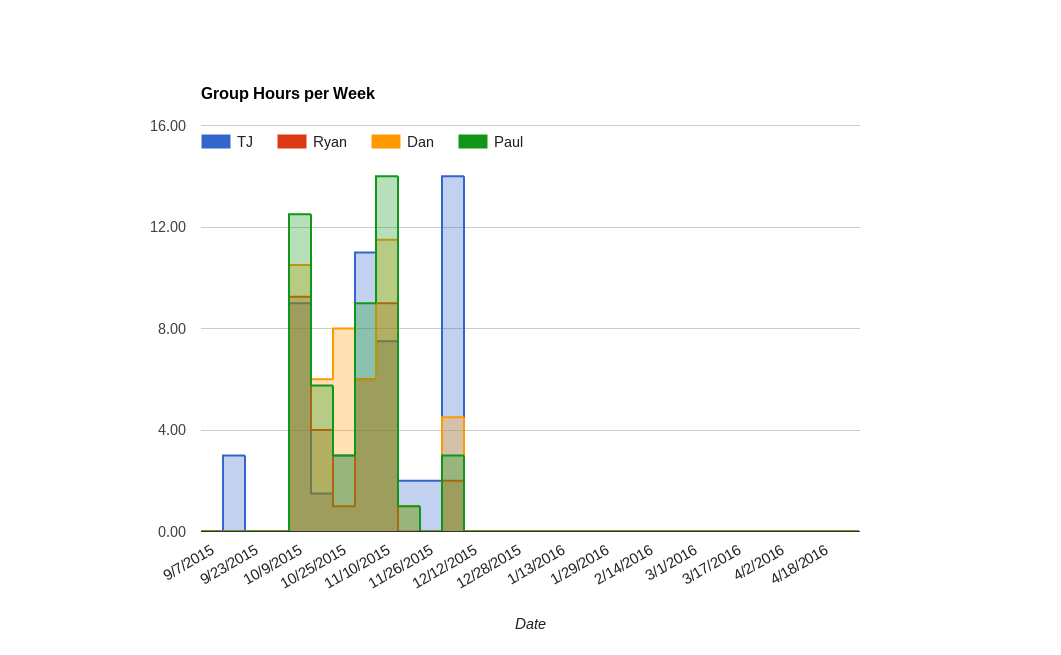
\includegraphics[width=\textwidth]{work_by_week.png}
    \caption{Work Done by Week}
    \label{fig:work_by_week}
\end{figure}

\end{document}
